\chapter{Resultados}

Neste capitulo serão apresentados e discutidos os resultados dos experimentos que buscam avaliar o MOEA-RS para recomendação de filmes, em comparação com um trabalho relacionado e com sistemas de recomendações tradicionais. Os resultados  podem ser visualizados na Tabela \ref{tab:main_results}, na Tabela, para cada medida de avaliação, são apresentados os valor médio a partir todas as recomendações feitas por cada método, o desvio padrão, a maior(e o menor) valor  obtido por cada método.

\begin{table}[h]

\centering
\begin{tabular}{r|l|cccr}Método & Medida & Precisão & \textit{Recall} & Diversidade & Novidade \\ 
\hline                               % para uma linha horizontal
MOEA-RS     & Média         & \textbf{0.949282} & 0.141767 & \textbf{0.201282} & \textbf{6.2386e-02} \\
            & Desvio Padrão & 0.105653 & 0.097391 & 0.156934 & 6.3856e-02 \\
            & Mínimo        & 0.000000 & 0.000000 & 0.000000 & 2.4023e-07 \\
            & Máximo        & 1.000000 & 0.900000 & 1.010196  & 1.4323e-01 \\
\hline  
CF          & Média         & 0.941084 & \textbf{0.274845} & 0.072433 &  6.2384e-02 \\
            & Desvio Padrão & 0.081718 & 0.138983 & 0.004091 & 6.3928e-02 \\
            & Mínimo        & 0.266667 & 0.025467 & 0.071429 & 2.8306e-07 \\
            & Máximo        & 1.000000 & 1.000000 & 0.097844 & 1.4316e-01 \\
\hline  
CB K-Means  & Média         & 0.896302 & 0.234154   & 0.111522 & 6.1519e-02\\
            & Desvio Padrão & 0.143168 & 0.147292   & 0.161155 & 6.1829e-02 \\
            & Mínimo        & 0.000000 & 0.000000   & 0.000000 & 2.5439e-07 \\
            & Máximo        & 1.000000 & 0.833333   & 1.004367 & 1.4326e-01 \\
\hline  
MOEA-D/RS   & Média         & 0.828279  & 0.194398 & 0.072255 & 6.2214e-02\\
            & Desvio Padrão & 0.167902  & 0.093568 & 0.003956 & 6.3908e-02\\
            & Mínimo        & 0.000000  & 0.000000 & 0.071429 & 2.5417e-07 \\
            & Máximo        & 1.000000  & 0.625000 & 0.131161 & 1.4315e-01 \\
\hline  
\end{tabular}
\caption{Variações selecionados para serem avaliados em conjunto com o MOEA-RS}
\label{tab:main_results}
\end{table}

Como pode ser visto na Tabela, o MOEA-RS superou o método com proposta relacionada (MOEA-D/RS) em todos os aspectos, com destaque para as medidas de precisão e diversidade, onde o MOEA-RS apresentou uma melhora de 14\%, para a medida de precisão, e 178\% para a medida de diversidade. 

Com relação aos métodos tradicionais(CF baseado em itens e CB-Kmeans), o MOEA-RS obteve melhores resultados para as medidas de precisão, diversidade e novidade, com destaque para medida de precisão, em que o MOEA-RS apresentou uma melhora de 0.8\% com relação ao CF baseado em itens, e para a medida de diversidade, que o MOEA-RS apresentou uma melhora de 80\% com relação ao CB K-Means.

Um dos motivos para MOEA-RS obter melhores resultados de precisão, com relação ao métodos tradicionais, foi o fato de que o MOEA-RS, apesar de ter uma maior quantidade de recomendações com valores precisão muito abaixo da média, como pode ser visto na Figura \ref{fig:boxplot_precision}, obteve valores de precisão máximo para uma quantidade usuários maior do que os outros métodos. Para proposito de comparação, o MOEA-RS obteve valor precisão máxima para 73\%, CF baseado em itens obteve o valor máximo para 50\% dos usuários e o CB-Kmeans 40\% .

\begin{figure}[h!]
   
    \centering
    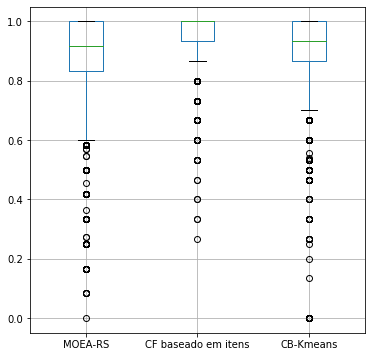
\includegraphics[width=14cm]{Imagens/precisions_boxplot.png}
   \caption{\textit{Boxplot} para os resultados relacionados a Precisão}
    \label{fig:boxplot_precision}
    
\end{figure}

Com relação as recomendações abaixo da média, como é apresentado na imagem acima a quantidade de usuários que tiveram recomendações do MOEA-RS, com uma precisão abaixo de 2 vezes o desvio padrão, é  pequeno quando comparado ao número total de usuário(aproximadamente 4.84\%), porém, esse valor é maior do que o CF baseado em itens que apenas 3.95\% dos usuários tiveram recomendações com precisão abaixo de 2 vezes o desvio padrão.  Na Tabela \ref{tab:low_precisions}, é apresentada as informações dos usuários que tiveram recomendações com precisão abaixo de 2 vezes o desvio padrão.

\begin{table}[H]
\centering
\begin{tabular}{|c| c | c c c |}
\hline
Informação      & Medida           & MOEA-RS    & CF-Item \\ 
\hline
Usuários        & Total             & 142       & 116\\
\hline
Tamanho do      & Média             & 187.5     & 149\\
conjunto de     & Desvio padrão     & 139.3     & 109\\
treino          & Mínimo            & 70        & 70\\
                & Máximo            & 734       & 661\\
\hline
Tamanho do      & Média             & 81        & 64\\
conjunto de     & Desvio padrão     & 59.6      & 46.7\\
teste           & Mínimo            & 30        & 30\\
                & Máximo            & 315       & 284\\
\hline
\end{tabular}
\caption{Informações sobre os usuários que tiveram recomendações com precisão abaixo de 0.5.}
\label{tab:low_precisions}
\end{table}

Outro fator que pode ser analisado nos resultados é a relação entre a quantidade de filmes utilizados no processo de recomendação e a precisão da recomendação, esse fator é importante para identificar se o MOEA-RS apresenta uma dificuldade que é comum em sistemas de recomendação, que é a baixa precisão na recomendações de itens para usuários com poucas avaliações. Na Tabela \ref{tab:cold_start}, pode ser visto a relação entre a quantidade de filmes e a precisão.



\begin{table}[H]
\centering
\begin{tabular}{|c| c | c c c |}
\hline
Quantidade de filmes    & Número de usuários    & MOEA-RS   & CF-Item\\ 
\hline
Entre  70 e 100         & 719                   & 0.942672  & 0.925359\\
\hline
Entre  100 e 150        & 725                   & 0.946123  & 0.938851\\
\hline
Entre  150 e 200        & 417                   & 0.949416  & 0.941966\\
\hline
Entre  200 e 300        & 504                   & 0.959696  & 0.953704\\
\hline
Entre  300 e 400        & 236                   & 0.949976  & 0.951130\\
\hline
Entre  400 e 800        & 256                   & 0.950488  & 0.954167\\
\hline
Entre  800 e 1613       & 26                    & 0.994505  & 0.969231\\
\hline
\end{tabular}
\caption{Relação entre a quantidade de filmes utilizados no processo de recomendação e a precisão da recomendação.}
\label{tab:all_precisions}
\end{table}

Como pode ser visto na Tabela acima, a quantidade de filmes avaliados pelos usuários influencia na precisão do MOEA-RS, mas a precisão recomendações para usuários com poucas avaliações foram maiores do que o CF baseado em itens.